\documentclass[12pt]{article}
\usepackage[utf8]{inputenc}
\usepackage[russian]{babel}
\usepackage[a4paper, vmargin=2cm, hmargin=1.5cm]{geometry}
\usepackage{amsmath}
\usepackage{tikz}
\usetikzlibrary{shapes, positioning, arrows}
\tikzstyle{elip}=[ellipse, draw, text width = {width("$S_{111111}$")}, align = center]
\usepackage{colortbl}
\usepackage{bm}
\usepackage{graphics}
\usepackage{booktabs}
\usepackage{multirow}
\usepackage{tabularx}

\usepackage{graphicx}
\graphicspath{{Paints/}}
\DeclareGraphicsExtensions{.pdf,.png,.jpg}

\newcolumntype{Y}{>{\centering\arraybackslash}X}

\begin{document}
	\begin{titlepage}
		\begin{center}
			\textbf{
				НАЦИОНАЛЬНЫЙ ИССЛЕДОВАТЕЛЬСКИЙ УНИВЕРСИТЕТ\\
				«ВЫСШАЯ ШКОЛА ЭКОНОМИКИ»\\
				Дисциплина: «Дискретная математика»\\
			}
			\vspace{5cm}
			\textbf{
				Домашнее задание 3\\
				\underline{Исследование алгоритмов решения}
				\\
				\underline{метрической задачи коммивояжера}
				\\
				Вариант 50\\
			}
		\end{center}
		\vspace{5cm}
		\begin{flushright}
			\textbf{
				Выполнила: Инкина Анастасия,\\
				студент гр. БПИ182.\\
				\vspace{5mm}
				Преподаватель: Дворянский Л.В.,\\
				Старший преподаватель\\
				программной инженерии\\
				факультета компьютерных наук\\
			}
		\end{flushright}
		\vspace{7cm}
		\begin{center}
			\textbf{Москва 2019}
		\end{center}
	\end{titlepage}

	\newpage
	\clearpage
	\setcounter{page}{2}
	\noindent
	1. На плоскости задано множество точек 
	$V = \{1, 2, 3, 4, 5, 6\}$
	своими координатами\\
        $(x_{1} = 8, y_{1} = 1), (x_{2} = 8, y_{2} = 2), (x_{3} = 9, y_{3} = 0), (x_{4} = 8, y_{4} = 4), (x_{5} = 9, y_{5} = 9), (x_{6} = 2, y_{6} = 1)$
        .\\

	%\input{input/vertices.tex}.
	
	\vspace{5mm}
	\noindent
	2. Вычислим элементы $d_{ij}$ весовой матрицы смежности графа
	$G = \langle V, V \times V \rangle$
	по формуле
	$$d_{ij} = |x_i - x_j| + |y_i - y_j|$$
	%\input{input/matrix1.tex}
\begin{flushleft}
$D$ =
$
\begin{pmatrix}
 0 & 1 & 2 & 3 & 9 & 6 \\
1 &  0 & 3 & 2 & 8 & 7 \\
2 & 3 &  0 & 5 & 9 & 8 \\
3 & 2 & 5 &  0 & 6 & 9 \\
9 & 8 & 9 & 6 &  0 & 15 \\
6 & 7 & 8 & 9 & 15 & 0 
\end{pmatrix}
$
\end{flushleft}
	
	\vspace{5mm}
	\noindent
	3. Используя метод ветвей и границ, найдем множество кодов всех оптимальных гамильтоновых циклов являющихся решением задачи коммивояжера на графе $G$.\\
	Петли не могут быть частью решения. Поэтому положим диагональные элементы равными бесконечности.\\
	%\input{input/matrix2.tex}

\begin{flushleft}
$D$ =
$
\begin{pmatrix}
 \infty & 1 & 2 & 3 & 9 & 6 \\
1 &  \infty & 3 & 2 & 8 & 7 \\
2 & 3 &  \infty & 5 & 9 & 8 \\
3 & 2 & 5 &  \infty & 6 & 9 \\
9 & 8 & 9 & 6 &  \infty & 15 \\
6 & 7 & 8 & 9 & 15 &  \infty 
\end{pmatrix}
$
\end{flushleft}

	
	Обозначим через
	$S = \{p:V \rightarrow V | (p(1) = 1) \&
	(\forall i \in V)(\forall j \in V)
	((p(i) = p(j)) \Rightarrow (i = j))\}$
	множество кодов всех гамильтоновых циклов
	$v = (p_1, p_2, p_3, p_4, p_5, p_6, p_1)$
	графа $G$, заданного весовой матрицей
	смежности $D$. Здесь $p_i$ используется
	в качестве сокращенной записи $p(i)$.\\
	Найдем нижнюю границу $b$ множества $S$\\



\begin{flushleft}
\begin{tabular}{c||rrrrrr||c}
S & 1 & 2 & 3 & 4 & 5 & 6 & \\
\hline
\hline
1 & $\infty$ & 1 & 2 & 3 & 9 & 6 & 1\\
2 & 1 & $\infty$ & 3 & 2 & 8 & 7 & 1\\
3 & 2 & 3 & $\infty$ & 5 & 9 & 8 & 2\\
4 & 3 & 2 & 5 & $\infty$ & 6 & 9 & 2\\
5 & 9 & 8 & 9 & 6 & $\infty$ & 15 & 6\\
6 & 6 & 7 & 8 & 9 & 15 & $\infty$ & 6\\
\hline
\hline
 &  &  &  &  & & $\alpha$ & 18\\
\end{tabular}
$\qquad $  
\begin{tabular}{c||rrrrrr||c}
S & 1 & 2 & 3 & 4 & 5 & 6 & \\
\hline
\hline
1 & $\infty$ & 0 & 1 & 2 & 8 & 5 & \\
2 & 0 & $\infty$ & 2 & 1 & 7 & 6 & \\
3 & 0 & 1 & $\infty$ & 3 & 7 & 6 & \\
4 & 1 & 0 & 3 & $\infty$ & 4 & 7 & \\
5 & 3 & 2 & 3 & 0 & $\infty$ & 9 & \\
6 & 0 & 1 & 2 & 3 & 9 & $\infty$ & $\beta$ \\
\hline
\hline
 & 0 & 0 & 1 & 0 & 4 & 5 & 2\\
\end{tabular}
\end{flushleft}

b = $\alpha$ + $\beta$ = 28

\begin{flushleft}
\begin{tabular}{c||rrrrrr||c}
S & 1 & 2 & 3 & 4 & 5 & 6 & \\
\hline
\hline
1 & $\infty$ & 0 & 0 & 2 & 4 & 0 & \\
2 & 0 & $\infty$ & 1 & 1 & 3 & 1 & \\
3 & 0 & 1 & $\infty$ & 3 & 3 & 1 & \\
4 & 1 & 0 & 2 & $\infty$ & 0 & 2 & \\
5 & 3 & 2 & 2 & 0 & $\infty$ & 4 & \\
6 & 0 & 1 & 1 & 3 & 5 & $\infty$ & \\
\hline
\hline
 &  &  &  &  & & & \\
\end{tabular}
\end{flushleft}

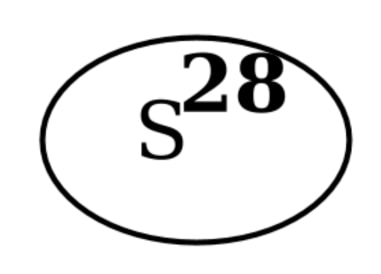
\includegraphics{picture_15}\\

Определим дугу ветвления для разбиения множества $S$

\begin{flushleft}
\begin{tabular}{c||rrrrrr||c}
S & 1 & 2 & 3 & 4 & 5 & 6 & \\
\hline
\hline
1 & $\infty$ & $0^0$ & $0^1$ & 2 & 4 & $0^1$ & \\
2 & $0^1$ & $\infty$ & 1 & 1 & 3 & 1 & \\
3 & $0^1$ & 1 & $\infty$ & 3 & 3 & 1 & \\
4 & 1 & $0^0$ & 2 & $\infty$ & $0^3$ & 2 & \\
5 & 3 & 2 & 2 & $0^3$ & $\infty$ & 4 & \\
    6 & $0^1$ & 1 & 1 & 3 & 5 & $\infty$ & \\
\hline
\hline
 &  &  &  &  & & & \\
\end{tabular}
\end{flushleft} 

Выбираем дугу $(5,4)$ 

\begin{flushleft}
\begin{tabular}{c||rrrrrr||c}
$S_0$ & 1 & 2 & 3 & 4 & 5 & 6 & \\
\hline
\hline
1 & $\infty$ & 0 & 0 & 2 & 4 & 0 & \\
2 & 0 & $\infty$ & 1 & 1 & 3 & 1 & \\
3 & 0 & 1 & $\infty$ & 3 & 3 & 1 & \\
4 & 1 & 0 & 2 & $\infty$ & 0 & 2 & \\
5 & 3 & 2 & 2 & $\colorbox{red}{$\infty$}$ & $\infty$ & 4 & 2\\
6 & 0 & 1 & 1 & 3 & 5 & $\infty$ & \\
\hline
\hline
 &  &  &  & 1 & &  & min\\
\end{tabular}
$\qquad $  
\begin{tabular}{c||rrrrrr||c}
$S_0$ & 1 & 2 & 3 & 4 & 5 & 6 & \\
\hline
\hline
1 & $\infty$ & 0 & 0 & 1 & 4 & 0 & \\
2 & 0 & $\infty$ & 1 & 0 & 3 & 1 & \\
3 & 0 & 1 & $\infty$ & 2 & 3 & 1 & \\
4 & 1 & 0 & 2 & $\infty$ & 0 & 2 & \\
5 & 1 & 0 & 0 & $\infty$ & $\infty$ & 2 \\
6 & 0 & 1 & 1 & 2 & 5 & $\infty$ & \\
\hline
\hline
 &  &  &  &  &  &  & \\
\end{tabular}
\end{flushleft}

$b_0$ = b + 3 = 31

\begin{flushleft}
\begin{tabular}{c||rrrrr||c}
$S_1$ & 1 & 2 & 3  & 5 & 6\\
\hline
\hline
1 & $\infty$ & 0 & 0  & 4 & 0 & \\
2 & 0 & $\infty$ & 1  & 3 & 1 & \\
3 & 0 & 1 & $\infty$  & 3 & 1 & \\
4 & 1 & 0 & 2  & $\colorbox{red}{$\infty$}$ & 2 & \\
6 & 0 & 1 & 1  & 5 & $\infty$ & \\
\hline
\hline
 &  &  &  & 3 & & min\\
\end{tabular}
$\qquad $  
\begin{tabular}{c||rrrrr||c}
$S_1$ & 1 & 2 & 3 & 4 & 5 & \\
\hline
\hline
1 & $\infty$ & 0 & 0  & 1 & 0 & \\
2 & 0 & $\infty$ & 1  & 0 & 1 & \\
3 & 0 & 1 & $\infty$  & 0 & 1 & \\
4 & 1 & 0 & 2  & $\infty$ & 2 & \\
6 & 0 & 1 & 1  & 2 & $\infty$ & \\
\hline
\hline
 & &  &  &  & & \\
\end{tabular}
\end{flushleft}

$b_1$ = b + 3 = 31\\

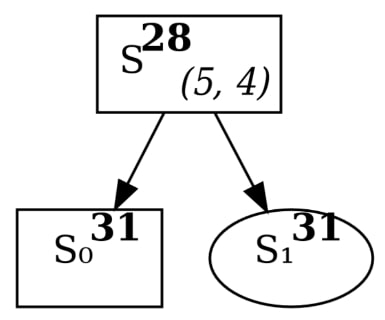
\includegraphics{picture_14}

Определим дугу ветвления для разбиения множества $S_1$

\begin{flushleft}
\begin{tabular}{c||rrrrr||c}
$S_1$ & 1 & 2 & 3 & 4 & 5 & \\
\hline
\hline
1 & $\infty$ & $0^0$ & $0^1$  & 1 & $0^1$ & \\
2 & $0^0$ & $\infty$ & 1  & $0^0$ & 1 & \\
3 & $0^0$ & 1 & $\infty$  & $0^0$ & 1 & \\
4 & 1 & $0^1$ & 2  & $\infty$ & 2 & \\
6 & $0^1$ & 1 & 1  & 2 & $\infty$ & \\
\hline
\hline
 & &  &  &  & & \\
\end{tabular}
\end{flushleft}

Выбираем дугу $(6,1)$ 

\begin{flushleft}
\begin{tabular}{c||rrrrr||c}
$S_{10}$ & 1 & 2 & 3 & 4 & 5 & \\
\hline
\hline
1 & $\infty$ & 0 & 0  & 1 & 0 & \\
2 & 0 & $\infty$ & 1  & 0 & 1 & \\
3 & 0 & 1 & $\infty$  & 0 & 1 & \\
4 & 1 & 0 & 2  & $\infty$ & 2 & \\
6 & $\colorbox{red}{$\infty$}$ & 1 & 1  & 2 & $\infty$ & 1\\
\hline
\hline
 &  &  &  &  & & min \\
\end{tabular}
$\qquad $  
\begin{tabular}{c||rrrrr||c}
$S_{10}$ & 1 & 2 & 3 & 4 & 5 & \\
\hline
\hline
1 & $\infty$ & 0 & 0  & 1 & 0 & \\
2 & 0 & $\infty$ & 1  & 0 & 1 & \\
3 & 0 & 1 & $\infty$  & 0 & 1 & \\
4 & 1 & 0 & 2  & $\infty$ & 2 & \\
    6 & $\infty$ & 0 & 0  & 1 & $\infty$ & \\
\hline
\hline
 & &  &  &  & & \\
\end{tabular}
\end{flushleft}

$b_{10}$ = $b_1$ + 1= 32

\begin{flushleft}
\begin{tabular}{c||rrrr||c}
$S_{11}$ & 2 & 3 & 4 & 5 & \\
\hline
\hline
1 &  0 & 0  & 1 & $\colorbox{red}{$\infty$}$ & \\
2 &  $\infty$ & 1  & 0 & 1 & \\
3 &  1 & $\infty$  & 0 & 1 & \\
4 &  0 & 2  & $\infty$ & 2 & \\
\hline
\hline
 &  &  &  &1 & min \\
\end{tabular}
$\qquad $  
\begin{tabular}{c||rrrr||c}
$S_{11}$ & 2 & 3 & 4 & 5 & \\
\hline
\hline
1 &  0 & 0  & 1 & $\infty$ & \\
2 &  $\infty$ & 1  & 0 & 0 & \\
3 &  1 & $\infty$  & 0 & 0 & \\
4 &  0 & 2  & $\infty$ & 1 & \\
\hline
\hline
 & &  &  & & \\
\end{tabular}
\end{flushleft}

$b_{11}$ = $b_1$ + 1= 32\\

%\includegraphics{123123}

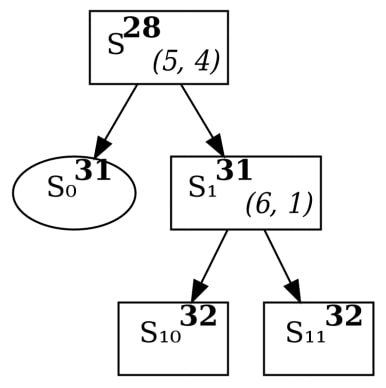
\includegraphics{picture_13}

Определим дугу ветвления для разбиения множества $S_0$\\

\begin{flushleft}
\begin{tabular}{c||rrrrrr||c}
$S_0$ & 1 & 2 & 3 & 4 & 5 & 6 & \\
\hline
\hline
1 & $\infty$ & $0^0$ & $0^0$ & 1 & 4 & $0^1$ & \\
2 & $0^0$ & $\infty$ & 1 & $0^0$ & 3 & 1 & \\
3 & $0^1$ & 1 & $\infty$ & 2 & 3 & 1 & \\
4 & 1 & $0^0$ & 2 & $\infty$ & $0^3$ & 2 & \\
5 & 1 & $0^0$ & $0^0$ & $\infty$ & $\infty$ & 2 \\
6 & $0^1$ & 1 & 1 & 2 & 5 & $\infty$ & \\
\hline
\hline
 &  &  &  &  &  &  & \\
\end{tabular}
\end{flushleft}

Выбираем дугу $(4,5)$

\begin{flushleft}
 \begin{tabular}{c||rrrrrr||c}
$S_{00}$ & 1 & 2 & 3 & 4 & 5 & 6 & \\
\hline
\hline
1 & $\infty$ & 0 & 0 & 1 & 4 & 0 & \\
2 & 0 & $\infty$ & 1 & 0 & 3 & 1 & \\
3 & 0 & 1 & $\infty$ & 2 & 3 & 1 & \\
4 & 1 & 0 & 2 & $\infty$ & $\colorbox{red}{$\infty$}$ & 2 & \\
5 & 1 & 0 & 0 & $\infty$ & $\infty$ & 2 \\
6 & 0 & 1 & 1 & 2 & 5 & $\infty$ & \\
\hline
\hline
 &  &  &  &  & 3 &  & min \\
\end{tabular}
$\qquad $  
\begin{tabular}{c||rrrrrr||c}
$S_{00}$ & 1 & 2 & 3 & 4 & 5 & 6 & \\
\hline
\hline
1 & $\infty$ & 0 & 0 & 1 & 1 & 0 & \\
2 & 0 & $\infty$ & 1 & 0 & 0 & 1 & \\
3 & 0 & 1 & $\infty$ & 2 & 0 & 1 & \\
4 & 1 & 0 & 2 & $\infty$ & $\infty$ & 2 & \\
5 & 1 & 0 & 0 & $\infty$ & $\infty$ & 2 \\
6 & 0 & 1 & 1 & 2 & 2 & $\infty$ & \\
\hline
\hline
 &  &  &  &  &  &  & \\
\end{tabular}
\end{flushleft}

$b_{00}$ = $b_0$ + 3= 34\\

\begin{flushleft}
 \begin{tabular}{c||rrrrr||c}
$S_{01}$ & 1 &2 & 3 & 4 & 6 & \\
\hline
\hline
1 & $\infty$ & 0 & 0 & 1  & 0 & \\
2 & 0 & $\infty$ & 1 & 0  & 1 & \\
3 & 0 & 1 & $\infty$ & 2  & 1 & \\
5 & 1 & 0 & 0 & $\infty$  & 2 \\
6 & 0 & 1 & 1 & 2 & $\infty$ & \\
\hline
\hline
 &  &   &  &  &  &  \\
\end{tabular}
\end{flushleft}

$b_{01}$ = $b_0$  = 31\\

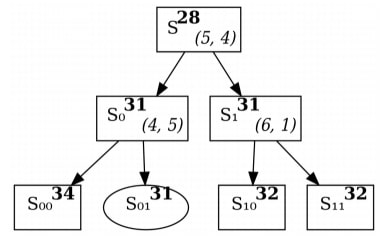
\includegraphics{picture_12}\\

Определим дугу ветвления для разбиения множества $S_{01}$\\

\begin{flushleft}
 \begin{tabular}{c||rrrrr||c}
$S_{01}$ & 1 &2 & 3 & 4 & 6 & \\
\hline
\hline
1 & $\infty$ & $0^0$ & $0^0$ & 1  & $0^1$ & \\
2 & $0^0$ & $\infty$ & 1 & $0^1$  & 1 & \\
3 & $0^1$ & 1 & $\infty$ & 2  & 1 & \\
5 & 1 & $0^0$ & $0^0$ & $\infty$  & 2 \\
6 & $0^1$ & 1 & 1 & 2 & $\infty$ & \\
\hline
\hline
 &  &   &  &  &  &  \\
\end{tabular}
\end{flushleft}

Выбираем дугу $(6,1)$

\begin{flushleft}
 \begin{tabular}{c||rrrrr||c}
$S_{010}$ & 1 &2 & 3 & 4 & 6 & \\
\hline
\hline
1 & $\infty$ & 0 & 0 & 1  & 0 & \\
2 & 0 & $\infty$ & 1 & 0  & 1 & \\
3 & 0 & 1 & $\infty$ & 2  & 1 & \\
5 & 1 & 0 & 0 & $\infty$  & 2 \\
6 & $\colorbox{red}{$\infty$}$ & 1 & 1 & 2 & $\infty$ & 1\\
\hline
\hline
 &  &   &  &  &  & min \\
\end{tabular}
$\qquad $ 
 \begin{tabular}{c||rrrrr||c}
$S_{010}$ & 1 &2 & 3 & 4 & 6 & \\
\hline
\hline
1 & $\infty$ & 0 & 0 & 1  & 0 & \\
2 & 0 & $\infty$ & 1 & 0  & 1 & \\
3 & 0 & 1 & $\infty$ & 2  & 1 & \\
5 & 1 & 0 & 0 & $\infty$  & 2 \\
6 & $\infty$ & 0 & 0 & 1 & $\infty$ & \\
\hline
\hline
 & &   &  &  &  & \\
\end{tabular}
\end{flushleft}

$b_{010}$ = $b_{01}$ + 1 = 32\\

\begin{flushleft}
\begin{tabular}{c||rrrr||c}
$S_{011}$  &2 & 3 & 4 & 6 & \\
\hline
\hline
1 &  0 & 0 & 1  & $\colorbox{red}{$\infty$}$ & \\
2 &  $\infty$ & 1 & 0  & 1 & \\
3 &  1 & $\infty$ & 2  & 1 & 1\\
5 &  0 & 0 & $\infty$  & 2 \\
\hline
\hline
 &  &  &  &  & min \\
\end{tabular}
$\qquad $ 
\begin{tabular}{c||rrrr||c}
$S_{011}$  &2 & 3 & 4 & 6 & \\
\hline
\hline
1 &  0 & 0 & 1  & $\infty$ & \\
2 &  $\infty$ & 1 & 0  & 1 & \\
3 &  0 & $\infty$ & 1  & 0 & \\
5 &  0 & 0 & $\infty$  & 2 \\
\hline
\hline
 &  &  &  & & \\
\end{tabular}
\end{flushleft}

$b_{011}$ = $b_{01}$ + 1 = 32\\

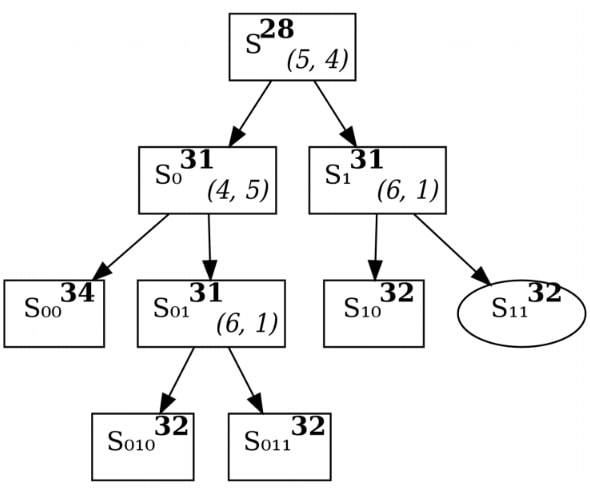
\includegraphics{picture_11}\\

Определим дугу ветвления для разбиения множества $S_{11}$\\

\begin{flushleft}
\begin{tabular}{c||rrrr||c}
$S_{11}$ & 2 & 3 & 5 & 6 & \\
\hline
\hline
1 &  $0^0$ & $0^1$  & 1 & $\infty$ & \\
2 &  $\infty$ & 1  & $0^0$ & $0^0$ & \\
3 &  1 & $\infty$  & $0^0$ & $0^0$ & \\
4 &  $0^1$ & 2  & $\infty$ & 1 & \\
\hline
\hline
 &  &  &  & & \\
\end{tabular}
\end{flushleft}

Выбираем дугу $(1,3)$

\begin{flushleft}
\begin{tabular}{c||rrrr||c}
$S_{110}$ & 2 & 3 & 5 & 6 & \\
\hline
\hline
1 &  0 & $\colorbox{red}{$\infty$}$  & 1 & $\infty$ & \\
2 &  $\infty$ & 1  & 0 & 0 & \\
3 &  1 & $\infty$  & 0 & 0 & \\
4 &  0 & 2  & $\infty$ & 1 & \\
\hline
\hline
 &  & 1 &  & & min \\
\end{tabular}
$\qquad $
\begin{tabular}{c||rrrr||c}
$S_{110}$ & 2 & 3 & 5 & 6 & \\
\hline
\hline
1 &  0 & $\infty$  & 1 & $\infty$ & \\
2 &  $\infty$ & 0  & 0 & 0 & \\
3 &  1 & $\infty$  & 0 & 0 & \\
4 &  0 & 1  & $\infty$ & 1 & \\
\hline
\hline
 &  &  &  & & \\
\end{tabular}
\end{flushleft}

$b_{0110}$ = $b_{11}$ + 1 = 32\\

\begin{flushleft}
\begin{tabular}{c||rrr||c}
    $S_{111}$ & 2  & 5 & 6 & \\
\hline
\hline
2 &  $\infty$   & 0 & 0 & \\
3 &  1   & 0 & $\colorbox{red}{$\infty$}$ & \\
4 &  0   & $\infty$ & 1 & \\
\hline
\hline
 &  &  &  & \\
\end{tabular}
\end{flushleft}

$b_{0111}$ = $b_{011}$ = 32\\

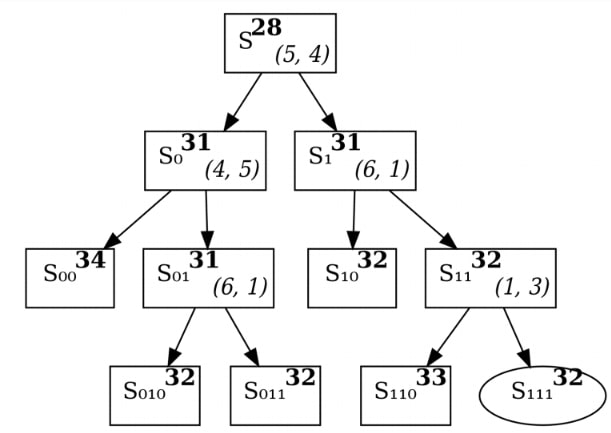
\includegraphics{picture_10}\\

Определим дугу ветвления для разбиения множества $S_{111}$\\

\begin{flushleft}
\begin{tabular}{c||rrr||c}
 $S_{111}$ & 2  & 5 & 6 & \\
\hline
\hline
2 &  $\infty$   & $0^0$ & $0^0$ & \\
3 &  1   & $0^1$ & $\infty$ & \\
4 &  $0^2$   & $\infty$ & 1 & \\
\hline
\hline
 &  &  &  & \\
\end{tabular}
\end{flushleft}

Выбираем дугу $(4,5)$

\begin{flushleft}
\begin{tabular}{c||rrr||c}
 $S_{1110}$ & 2  & 5 & 6 & \\
\hline
\hline
2 &  $\infty$ &0& 0 & \\
3 &  1   & 0 & $\infty$ & \\
4 &  $\colorbox{red}{$\infty$}$   & $\infty$ & 1 & 1\\
\hline
\hline
 & 1 &  &  & min \\
\end{tabular}
$\qquad $ 
\begin{tabular}{c||rrr||c}
 $S_{1110}$ & 2  & 5 & 6 & \\
\hline
\hline
2 &  $\infty$ &0& 0 & \\
3 &  0   & 0 & $\infty$ & \\
4 &  $\infty$  & $\infty$ & 0 & \\
\hline
\hline
 & &  &  & \\
\end{tabular}
\end{flushleft}

$b_{1110}$ = $b_{111}$ + 2 = 34\\

\begin{flushleft}
\begin{tabular}{c||rr||c}
 $S_{1111}$ & 2   & 6 & \\
\hline
\hline
2 &  $\infty$ & 0 & \\
3 &  0   &  $\infty$ & \\
\hline
\hline
 & &  & \\
\end{tabular}
\end{flushleft}

$b_{1111}$ = $b_{111}$ = 32\\

v = (1, 3, 5, 4, 2, 6, 1), $f(v)$ = $b_{1111}$  = 32\\

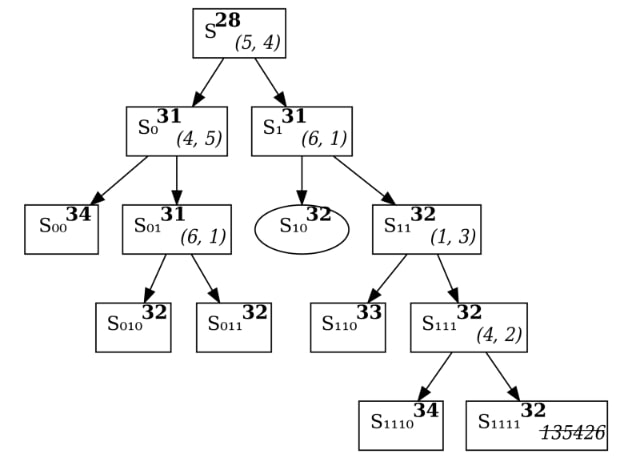
\includegraphics{picture_09}\\

Определим дугу ветвления для разбиения множества $S_{10}$\\

\begin{flushleft}
\begin{tabular}{c||rrrrr||c}
$S_{10}$ & 1 & 2 & 3 & 5 & 6 & \\
\hline
\hline
1 & $\infty$ & $0^0$ & $0^0$  & 1 & $0^1$ & \\
2 & $0^0$ & $\infty$ & 1  & $0^0$ & 1 & \\
3 & $0^0$ & 1 & $\infty$  & $0^0$ & 1 & \\
4 & 1 & $0^1$ & 2  & $\infty$ & 2 & \\
6 & $\infty$ & $0^0$ & $0^0$  & 1 & $\infty$ & \\
\hline
\hline
 &  &  &  &  & \\
\end{tabular}
\end{flushleft}

Выбираем дугу $(1,6)$

\begin{flushleft}
\begin{tabular}{c||rrrrr||c}
$S_{100}$ & 1 & 2 & 3 & 5 & 6 & \\
\hline
\hline
1 & $\infty$ & 0 & 0  & 1 & $\colorbox{red}{$\infty$}$ & \\
2 & 0 & $\infty$ & 1  & 0 & 1 & \\
3 & 0 & 1 & $\infty$  & 0 & 1 & \\
4 & 1 & 0 & 2  & $\infty$ & 2 & \\
6 & $\infty$ & 0 & 0  & 1 & $\infty$ & \\
\hline
\hline
 &  &   &    & 1 &  & min \\
\end{tabular}
$\qquad $ 
\begin{tabular}{c||rrrrr||c}
$S_{100}$ & 1 & 2 & 3 & 5 & 6 & \\
\hline
\hline
1 & $\infty$ & 0 & 0  & 1 & $\infty$ & \\
2 & 0 & $\infty$ & 1  & 0 & 0 & \\
3 & 0 & 1 & $\infty$  & 0 & 0 & \\
4 & 1 & 0 & 2  & $\infty$ & 1 & \\
6 & $\infty$ & 0 & 0  & 1 & $\infty$ & \\
\hline
\hline
 &  &  &  &  &  & \\
\end{tabular}
\end{flushleft}

$b_{100}$ = $b_{10}$ + 1 = 33\\

\begin{flushleft}
\begin{tabular}{c||rrrr||c}
$S_{101}$ & 1 & 2 & 3 & 5 &  \\
\hline
\hline
2 & 0 & $\infty$ & 1  & 0 &  \\
3 & 0 & 1 & $\infty$  & 0 &  \\
4 & 1 & 0 & 2  & $\infty$ &  \\
6 & $\infty$ & 0 & 0  & 1 &  \\
\hline
\hline
 &  &  &  &  &   \\
\end{tabular}
\end{flushleft}

$b_{101}$ = $b_{10}$= 32\\

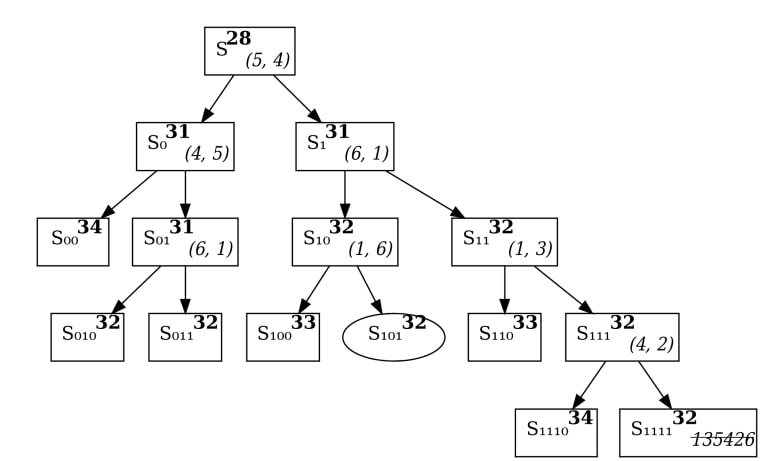
\includegraphics{picture_08}\\



Определим дугу ветвления для разбиения множества $S_{101}$\\

\begin{flushleft}
\begin{tabular}{c||rrrr||c}
$S_{101}$ & 1 & 2 & 3 & 5 &  \\
\hline
\hline
2 & $0^0$ & $\infty$ & 1  & $0^0$ &  \\
3 & $0^0$ & 1 & $\infty$  & $0^0$ &  \\
4 & 1 & $0^1$ & 2  & $\infty$ &  \\
6 & $\infty$ & $0^0$ & $0^1$  & 1 &  \\
\hline
\hline
 &  &    &  & \\
\end{tabular}
\end{flushleft}

Выбираем дугу $(6,3)$

\begin{flushleft}
\begin{tabular}{c||rrrr||c}
$S_{1010}$ & 1 & 2 & 3 & 5 &  \\
\hline
\hline
2 & 0 & $\infty$ & 1  & 0 &  \\
3 & 0 & 1 & $\infty$  & 0 &  \\
4 & 1 & 0 & 2  & $\infty$ &  \\
6 & $\infty$ & 0 & $\colorbox{red}{$\infty$}$ & 1 &  \\
\hline
\hline
  &  1&  &  & &min \\
\end{tabular}
$\qquad $ 
\begin{tabular}{c||rrrr||c}
$S_{1010}$ & 1 & 2 & 3 & 5 &  \\
\hline
\hline
2 & 0 & $\infty$ & 0         & 0 &  \\
3 & 0 &        1 & $\infty$  & 0 &  \\
4 & 1 &        0 & 1         & $\infty$ &  \\
6 & $\infty$ & 0 & $\infty$  & 1 &  \\
\hline
\hline
     &  &  &  & \\
\end{tabular}
\end{flushleft}

$b_{1010}$ = $b_{101}$  = 32\\

\begin{flushleft}
\begin{tabular}{c||rrr||c}
$S_{1011}$ & 1 & 2  & 5 &  \\
\hline
\hline
2 & 0 & $\infty$   & 0 &  \\
3 & $\colorbox{red}{$\infty$}$ & 1   & 0 &  \\
4 & 1 & 0   & $\infty$ &  \\
\hline
\hline
  &  &  & \\
\end{tabular}
\end{flushleft}

$b_{1011}$ = $b_{101}$= 32\\

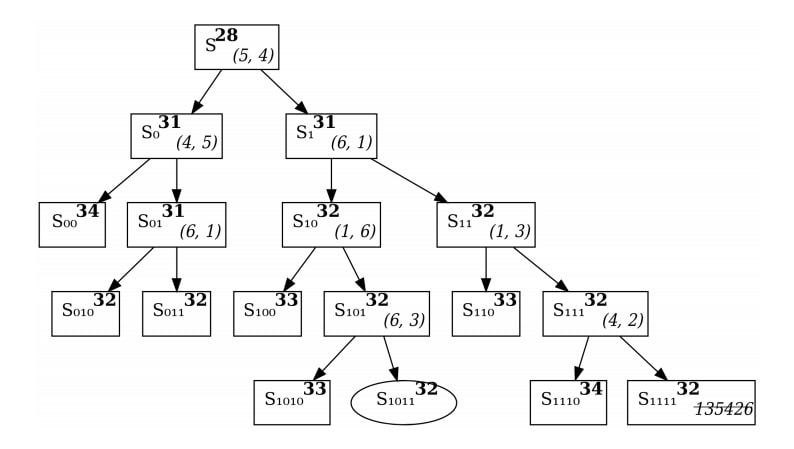
\includegraphics{picture_07}\\ 


% 1 point
Определим дугу ветвления для разбиения множества $S_{1011}$\\

\begin{flushleft}
\begin{tabular}{c||rrr||c}
$S_{1011}$ & 1 & 2  & 5 &  \\
\hline
\hline
2 & $0^1$ & $\infty$   & $0^0$ &  \\
3 & $\infty$ & 1   & $0^1$ &  \\
4 & 1 & $0^2$   & $\infty$ &  \\
\hline
\hline
 &  &  &  &  & \\
\end{tabular}
\end{flushleft}

Выбираем дугу $(4,2)$

\begin{flushleft}
\begin{tabular}{c||rrr||c}
$S_{10110}$ & 1 & 2  & 5 &  \\
\hline
\hline
2 & 0 & $\infty$   & 0 &  \\
3 & $\infty$ & 1   & 0 &  \\
4 & 1 & $\colorbox{red}{$\infty$}$   & $\infty$ &  1\\
\hline
\hline
 &  & 1     && min \\
\end{tabular}
$\qquad $ 
\begin{tabular}{c||rrr||c}
$S_{10110}$ & 1 & 2  & 5 &  \\
\hline
\hline
2 & 0 & $\infty$   & 0 &  \\
3 & $\infty$ & 0   & 0 &  \\
4 & 0 & $\infty$   & $\infty$ & \\
\hline
\hline
 &  &    & \\
\end{tabular}
\end{flushleft}

$b_{10110}$ = $b_{1011}$ + 2 = 34\\

\begin{flushleft}
\begin{tabular}{c||rr||c}
$S_{10111}$ & 1   & 5 &  \\
\hline
\hline
2 & 0 &  $\colorbox{red}{$\infty$}$ &  \\
3 & $\infty$    & 0 &  \\
\hline
\hline
     &  & \\
\end{tabular}
\end{flushleft}

$b_{10111}$ = $b_{1011}$ = 32\\

v = (1, 6, 3, 5, 4, 2, 1), $f(v)$ = $b_{10111}$  = 32\\
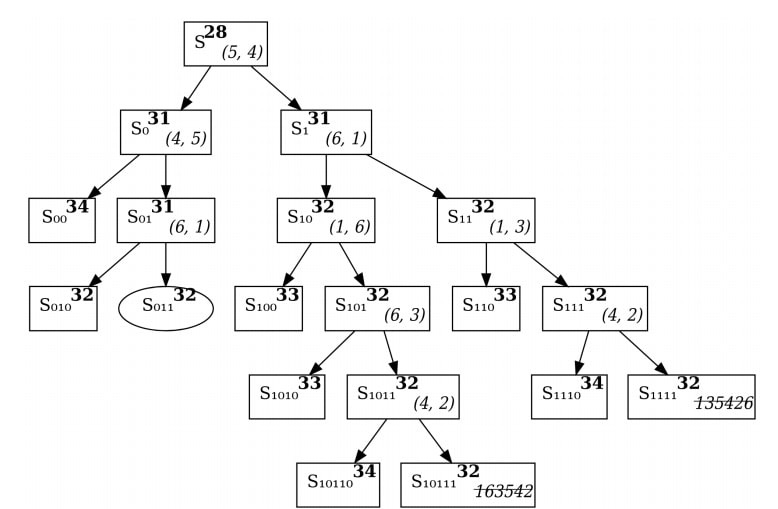
\includegraphics{picture_06}\\ 

% 2 point copy хыыы

Определим дугу ветвления для разбиения множества $S_{011}$\\

\begin{flushleft}
\begin{tabular}{c||rrrr||c}
$S_{011}$  &2 & 3 & 4 & 6 & \\
\hline
\hline
1 &  $0^0$ & $0^0$ & 1  & $\infty$ & \\
2 &  $\infty$ & 1 & $0^2$  & 1 & \\
3 &  $0^0$ & $\infty$ & 1  & $0^1$ & \\
5 &  $0^0$ & $0^0$ & $\infty$  & 2 \\
\hline
\hline
 &  &  &  & \\
\end{tabular}
\end{flushleft}

Выбираем дугу $(2,4)$

\begin{flushleft}
\begin{tabular}{c||rrrr||c}
$S_{0110}$  &2 & 3 & 4 & 6 & \\
\hline
\hline
1 &  0        & 0        & 1                           & $\infty$ & \\
2 &  $\infty$ & 1        & $\colorbox{red}{$\infty$}$  & 1 & 1\\
3 &  0        & $\infty$ & 1                           & 0 & \\
5 &  0        & 0        & $\infty$                    & 2 & \\
\hline
\hline
 &  &  & 1 && min \\
\end{tabular}
$\qquad $ 
\begin{tabular}{c||rrrr||c}
$S_{0110}$  &2 & 3 & 4 & 6 & \\
\hline
\hline
1 &  0        & 0        & 0                           & $\infty$ & \\
2 &  $\infty$ & 0        & $\infty$  & 0 & \\
3 &  0        & $\infty$ & 0                           & 0 & \\
5 &  0        & 0        & $\infty$                    & 2 & \\
\hline
\hline
 &  &  &  & \\
\end{tabular}
\end{flushleft}

$b_{0110}$ = $b_{011}$ + 2 = 34\\

\begin{flushleft}
\begin{tabular}{c||rrr||c}
$S_{0111}$  &2 & 3 &  6 & \\
\hline
\hline
1 &  0        & 0           & $\infty$ & \\
3 &  0        & $\infty$    & 0 & \\
5 &  $\colorbox{red}{$\infty$}$        & 0           & 2 & \\
\hline
\hline
 &    &  & &  \\
\end{tabular}
\end{flushleft}
$b_{0111}$ = $b_{011}$ = 32\\

v = (1, 3, 4, 5, 2, 6, 1), $f(v)$ = $b_{001111}$  = 20\\

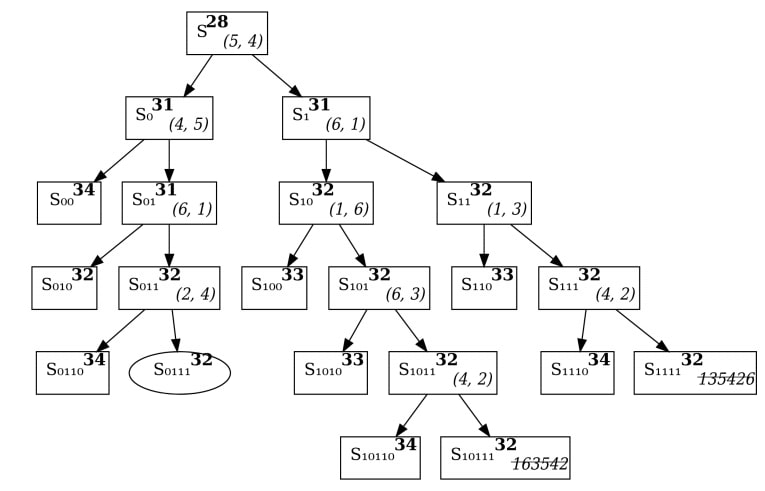
\includegraphics{picture_05}\\ 


% Похнали копи и S11

Определим дугу ветвления для разбиения множества $S_{0111}$\\

\begin{flushleft}
\begin{tabular}{c||rrr||c}
$S_{0111}$  &2 & 3 &  6 & \\
\hline
\hline
1 &  $0^0$        & $0^0$           & $\infty$ & \\
3 &  $0^0$        & $\infty$    & $0^0$ & \\
5 &  $\infty$        & $0^0$           & 2 & \\
\hline
\hline
 &  &  & &  \\
\end{tabular}
\end{flushleft}

Выбираем дугу $(5,3)$

\begin{flushleft}
\begin{tabular}{c||rrr||c}
$S_{01110}$  &2 & 3 &  6 & \\
\hline
\hline
1 &  0        & 0           & $\infty$ & \\
3 &  0        & $\infty$    & 0 & \\
5 &  $\infty$        & $\colorbox{red}{$\infty$}$           & 2 & 2\\
\hline
\hline
 &  &  &  & min  \\
\end{tabular}
$\qquad $ 
\begin{tabular}{c||rrr||c}
$S_{01110}$  &2 & 3 &  6 & \\
\hline
\hline
1 &  0        & 0           & $\infty$ & \\
3 &  0        & $\infty$    & 0 & \\
5 &  $\infty$        & $\infty$           & 0 &  \\
\hline
\hline
 &  &  & & \\
\end{tabular}
\end{flushleft}

$b_{01110}$ = $b_{0111}$ + 2 = 34\\

\begin{flushleft}
\begin{tabular}{c||rr||c}
$S_{01111}$  &2  &  6 & \\
\hline
\hline
1 &  0                   & $\infty$ & \\
3 &  $\colorbox{red}{$\infty$}$            & 0 & \\
\hline
\hline
 & & & \\
\end{tabular}
\end{flushleft}

$b_{01111}$ = $b_{0111}$  = 32\\


v = (1, 2, 4, 5, 3, 6, 1), $f(v)$ = $b_{01111}$  = 32\\

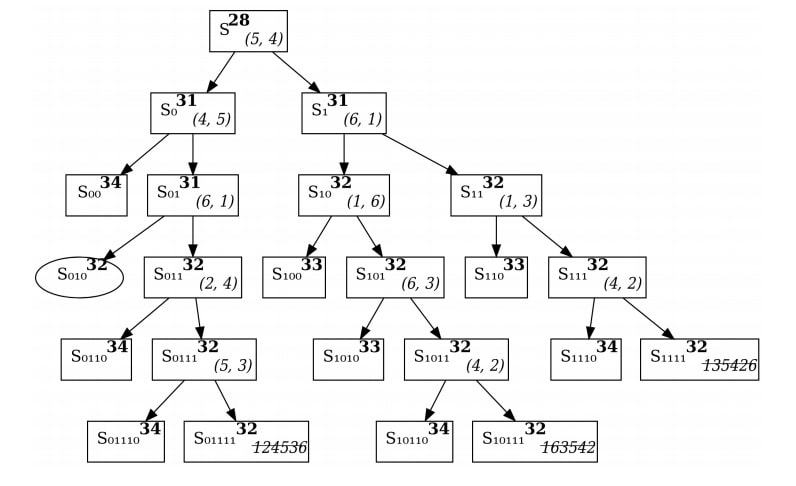
\includegraphics{picture_04}\\ 


% Похнали копи и S111

Определим дугу ветвления для разбиения множества $S_{010}$\\

\begin{flushleft}
 \begin{tabular}{c||rrrrr||c}
$S_{010}$ & 1 &2 & 3 & 4 & 6 & \\
\hline
\hline
1 & $\infty$ & $0^0$ & $0^0$ & 1  & $0^1$ & \\
2 & $0^0$ & $\infty$ & 1 & $0^1$  & 1 & \\
3 & $0^1$ & 1 & $\infty$ & 2  & 1 & \\
5 & 1 & $0^0$ & $0^0$ & $\infty$  & 2 \\
6 & $\infty$ & $0^0$ & $0^0$ & 1 & $\infty$ & \\
\hline
\hline
 & &   &  &  &  & \\
\end{tabular}
\end{flushleft}

Выбираем дугу $(2,4)$

\begin{flushleft}
 \begin{tabular}{c||rrrrr||c}
$S_{0100}$ & 1 &2 & 3 & 4 & 6 & \\
\hline
\hline
1 & $\infty$ & 0 & 0 & 1  & 0 & \\
2 & 0 & $\infty$ & 1 & $\colorbox{red}{$\infty$}$  & 1 & \\
3 & 0 & 1 & $\infty$ & 2  & 1 & \\
5 & 1 & 0 & 0 & $\infty$  & 2 \\
6 & $\infty$ & 0 & 0 & 1 & $\infty$ & \\
\hline
\hline
 & &   &  & 1 &  &min \\
\end{tabular}
$\qquad $ 
 \begin{tabular}{c||rrrrr||c}
$S_{0100}$ & 1 &2 & 3 & 4 & 6 & \\
\hline
\hline
1 & $\infty$ & 0 & 0 & 0  & 0 & \\
2 & 0 & $\infty$ & 1 & $\infty$  & 1 & \\
3 & 0 & 1 & $\infty$ & 1  & 1 & \\
5 & 1 & 0 & 0 & $\infty$  & 2 \\
6 & $\infty$ & 0 & 0 & 0 & $\infty$ & \\
\hline
\hline
 & &   &  &  &  & \\
\end{tabular}
\end{flushleft}

$b_{0100}$ = $b_{010}$ + 1 = 33\\

\begin{flushleft}
 \begin{tabular}{c||rrrr||c}
$S_{0101}$ & 1 &2 & 3  & 6 & \\
\hline
\hline
1 & $\infty$ & 0 & 0   & 0 & \\
3 & 0 & 1 & $\infty$   & 1 & \\
5 & 1 &  $\colorbox{red}{$\infty$}$ &  0 & 2 &\\
6 & $\infty$ & 0 & 0  & $\infty$ & \\
\hline
\hline
 & &   &  &   & \\
\end{tabular}
\end{flushleft}

$b_{0101}$ = $b_{010}$ = 32\\

v = (1, 6, 3, 4, 5, 2, 1), $f(v)$ = $b_{1111}$  = 20\\

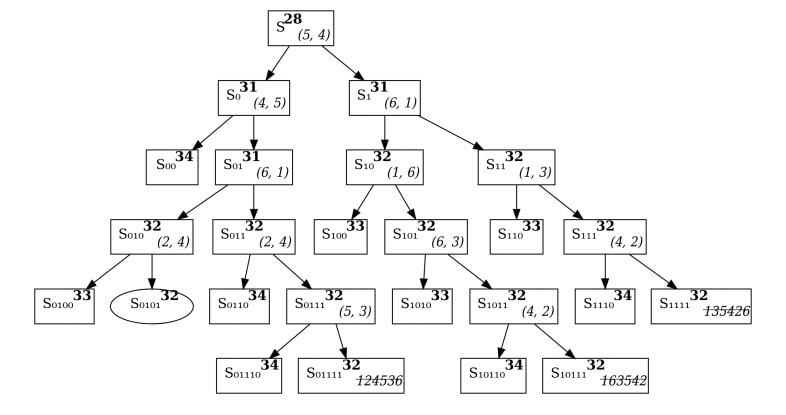
\includegraphics{picture_03}\\\\\\\\\\



% Похнали копи и S10

Определим дугу ветвления для разбиения множества $S_{0101}$\\

\begin{flushleft}
 \begin{tabular}{c||rrrr||c}
$S_{0101}$ & 1 &2 & 3  & 6 & \\
\hline
\hline
1 & $\infty$ & $0^0$ & $0^0$   & $0^1$ & \\
3 & $0^2$ & 1 & $\infty$   & 1 & \\
5 & 1 &  $\infty$ &  $0^1$ & 2 &\\
6 & $\infty$ & $0^0$ & $0^0$  & $\infty$ & \\
\hline
\hline
 & &   &  &   & \\
\end{tabular}
\end{flushleft}

Выбираем дугу $(3,1)$

\begin{flushleft}
 \begin{tabular}{c||rrrr||c}
$S_{01010}$ & 1 &2 & 3  & 6 & \\
\hline
\hline
1 & $\infty$ & 0 & 0   & 0 & \\
3 & $\colorbox{red}{$\infty$}$ & 1 & $\infty$   & 1 & 1\\
5 & 1 &  $\infty$ &  0 & 2 &\\
6 & $\infty$ & 0 & 0  & $\infty$ & \\
\hline
\hline
 & &   &  &   &min \\
\end{tabular}
$\qquad $ 
 \begin{tabular}{c||rrrr||c}
$S_{01010}$ & 1 &2 & 3  & 6 & \\
\hline
\hline
1 & $\infty$ & 0 & 0   & 0 & \\
3 & $\infty$ & 0 & $\infty$   & 0 & \\
5 & 1 &  $\infty$ &  0 & 2 &\\
6 & $\infty$ & 0 & 0  & $\infty$ & \\
\hline
\hline
 & &   &  &   & \\
\end{tabular}
\end{flushleft}

$b_{01010}$ = $b_{0101}$ + 1 = 33\\

\begin{flushleft}
 \begin{tabular}{c||rrr||c}
$S_{01011}$  &2 & 3  & 6 & \\
\hline
\hline
1 & 0 & $\colorbox{red}{$\infty$}$ & 0 & \\
5 & $\infty$ &  0 & 2 &\\
6 & 0 & 0  & $\infty$ & \\
\hline
\hline
 & &  &   & \\
\end{tabular}
\end{flushleft}

$b_{01011}$ = $b_{0101}$ = 32\\

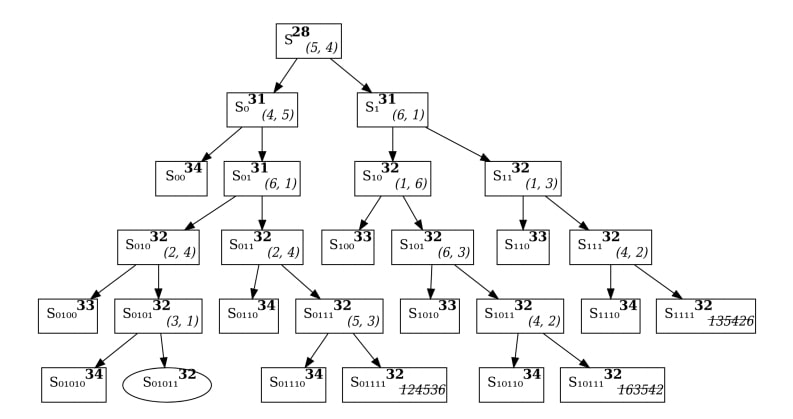
\includegraphics{picture_02}\\ 


% Похнали копи и S101

Определим дугу ветвления для разбиения множества $S_{01011}$\\

\begin{flushleft}
 \begin{tabular}{c||rrr||c}
$S_{01011}$  &2 & 3  & 6 & \\
\hline
\hline
1 & $0^0$ & $\infty$ & $0^2$ & \\
5 & $\infty$ &  $0^2$ & 2 &\\
6 & $0^0$ & $0^0$  & $\infty$ & \\
\hline
\hline
 & &  &   & \\
\end{tabular}
\end{flushleft}

Выбираем дугу $(5,3)$

\begin{flushleft}
 \begin{tabular}{c||rrr||c}
$S_{010110}$  &2 & 3  & 6 & \\
\hline
\hline
1 & 0 & $\infty$ & 0 & \\
5 & $\infty$ & $\colorbox{red}{$\infty$}$ & 2 &2\\
6 & 0 & 0  & $\infty$ & \\
\hline
\hline
 & &  &   &min \\
\end{tabular}
$\qquad $ 
 \begin{tabular}{c||rrr||c}
$S_{010110}$  &2 & 3  & 6 & \\
\hline
\hline
1 & 0 & $\infty$ & 0 & \\
5 & $\infty$ & $\infty$ & 0 &\\
6 & 0 & 0  & $\infty$ & \\
\hline
\hline
 & &  &   & \\
\end{tabular}
\end{flushleft}

$b_{010110}$ = $b_{01011}$ + 2 = 34\\

\begin{flushleft}
 \begin{tabular}{c||rr||c}
$S_{010111}$  &2   & 6 & \\
\hline
\hline
1 & $\colorbox{red}{$\infty$}$      & 0 & \\
6 & 0   & $\infty$ & \\
\hline
\hline
  &   & \\
\end{tabular}
\end{flushleft}

$b_{010111}$ = $b_{01011}$  = 32\\



v = (1, 6, 2, 4, 5, 3, 1), $f(v)$ = $b_{010111}$  = 32\\

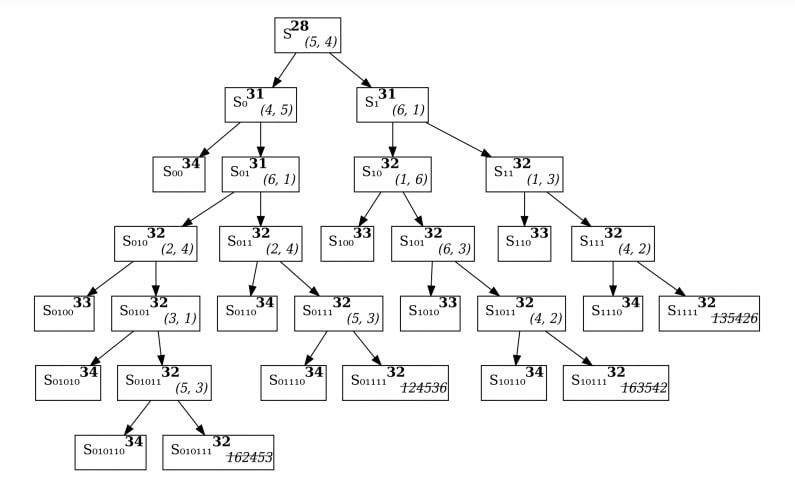
\includegraphics{picture_01} 

	\noindent
	\textbf{Ответ:} множество кодов всех оптимальных гамильтоновых 
	циклов являющихся решением задачи коммивояжера на графе $G$ есть 
	\{1354261, 1635421, 1245361, 1624531\}.
	Вес $f_0$ оптимального гамильтонова цикла равен $32$. \\
	
	4. Используя весовую матрицу смежности $D$ графа $G$,
	построим кратчайшее связывающее дерево T волновым методом. \\


\begin{tabular}{@{}|c|c|c|c|c|c|c|c|c|c|c|c|@{}}
\toprule
\multicolumn{2}{|c|}{1}                 & \multicolumn{2}{c|}{2}                 & \multicolumn{2}{c|}{3} & \multicolumn{2}{c|}{4} & \multicolumn{2}{c|}{5}                 & \multicolumn{2}{c|}{6}                 \\ \midrule
L                  & W                  & L                  & W                 & L          & W         & L          & W         & L                  & W                 & L                  & W                 \\ \midrule
0                  & 0                  & $\infty$                 & 0                 & $\infty$         & 0         & $\infty$         & 0         & $\infty$                 & 0                 & $\infty$                 & 0                 \\ \midrule
\multicolumn{2}{|c|}{\multirow{4}{*}{}} & 2                  & 1                 & 7          & 1         & 8          & 1         & 5                  & 1                 & 0                  & 1                 \\ \cmidrule(l){3-12} 
\multicolumn{2}{|c|}{}                  & \multicolumn{2}{c|}{\multirow{3}{*}{}} & \multicolumn{2}{c|}{}  & 6          & 2         & 3                  & 2                 & \multicolumn{2}{c|}{\multirow{3}{*}{}} \\ \cmidrule(lr){5-10}
\multicolumn{2}{|c|}{}                  & \multicolumn{2}{c|}{}                  & 6          & 5         & 3          & 5         & \multicolumn{2}{c|}{\multirow{2}{*}{}} & \multicolumn{2}{c|}{}                  \\ \cmidrule(lr){5-8}
\multicolumn{2}{|c|}{}                  & \multicolumn{2}{c|}{}                  & 5          & 4         & \multicolumn{2}{c|}{}  & \multicolumn{2}{c|}{}                  & \multicolumn{2}{c|}{}                  \\ \bottomrule
\end{tabular}

	$E(T) = \{(2, 1), (4, 2), (3, 4), (6, 3), (5, 6)\}$
	Вес дерева 
	$f(T) = \sum\limits_{(i, j) \in E(T)} d_{ij} = \sum\limits_{i = 1}^6 \lambda_{i} = 31$ \\ \\
	
	\noindent
	5. Найдем приближенное значение задачи коммивояжера $v_1$
	с помощью первого алгоритма \\ Кристофидеса. \\
	В графе с удвоенным числом ребер дерева \\
	$E(T)||E(T) = \{(2, 1), (1, 2), (3, 4), (4, 3), (4, 2), (2, 4), (5, 6), (6, 5), (6, 3), (3, 6)\}$ \\
	Построим Эйлеров цикл $\mu = (1, 2, 4, 3, 6, 5, 6, 3, 4, 2 ,1)$. \\
	Удалим повторения вершин в Эйлеровом цикле для получения 
	приближенного решения \\
	$v_1 = (1, 2, 4, 3, 6, 5, 1)$.
	Вес полученного гамильтонова цикла равен \\
	$f(v_1) = 1 + 2 + 5 + 8 + 15 + 9 = 40$ \\
	Вычислим относительную точность полученного решения
	$\epsilon = \frac{f(v_1) - f(v_0)}{f(v_0)} = \frac{40 - 32}{32} = 0.25$ \\
	Таким образом, найдено приближенное решение задачи коммивояжера. \\ \\
	
	\noindent
	6. Найдем приближенное решение задачи коммивояжера $v_2$ 
	с помощью второго алгоритма \\ Кристофидеса. \\
	Кратчайшее связывающее дерево имеет ребра
	$E(T) = \{(2, 1), (4, 2), (3, 4), (6, 3), (5, 6)\}$ \\
	В дереве две вершины нечетной степени: 1 и 5.
	\\ В оптимальное паросочетание $E(M) = \{(1, 5)\}$ 
	входит единственное ребро. \\
     Строим Эйлеров цикл в графе со множеством ребер \\
	$E(T) || E(M) = \{(1, 5), (2, 1), (4, 2), (3, 4), (6, 3), (5, 6)\}$ \\
	Полученный эйлеров цикл является одновременно и гамильтоновым \\
	$v_2 = \mu =  (5, 1, 2, 4, 3, 6, 5)$
	Вес полученного гамильтонова цикла равен \\
	$f(v_2) = 9 + 1 + 2 + 5 + 8 + 15 = 40$ \\
	Вычислим относительную точность полученного решения
	$\epsilon = \frac{f(v_2) - f(v_0)}{f(v_0)} = \frac{40 - 32}{32} = 0.25$ \\
	Таким образом, найдено приближенное решение задачи коммивояжера. \\ \\
\end{document} 